\chapter{研究目的}
%
\section{分類対象}
今回対象とする情報は,SNS上で投稿された画像つきで発信されたニュースである.
そのなかでも,正しいニュースを発信していたもの,フェイクニュースを発信していたもの,ジョークニュースを発信していたものが対象となる.
それぞれの例を今回扱ったデータセットから抜粋したものが以下の図\ref{fig:examples}である.

\begin{figure}[h]
    \centering
    \begin{subfigure}{0.31\textwidth}
        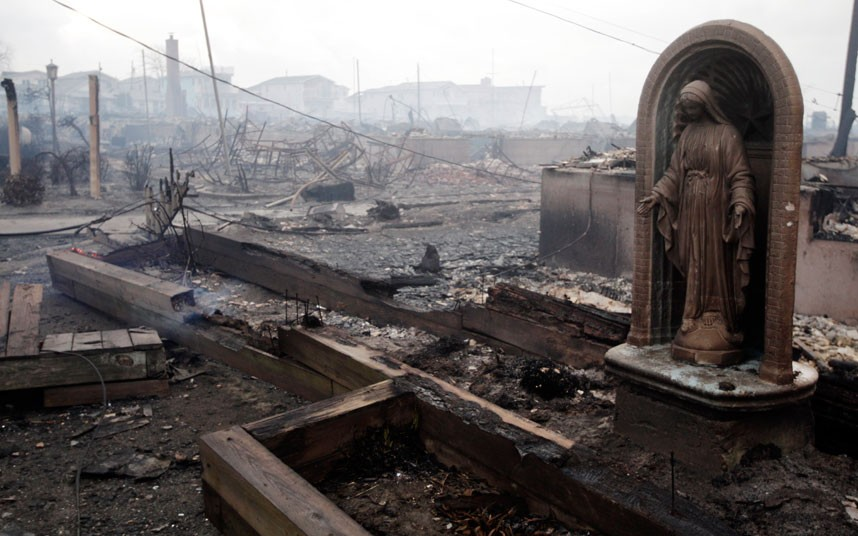
\includegraphics[width=\linewidth]{images/real_example.jpg}
        \caption{Recovering From Sandy: Breezy Point, Queens; Santiago, Cuba}
        \label{fig:real}
    \end{subfigure}
    \hspace*{\fill} % separation between the subfigures
    \begin{subfigure}{0.31\textwidth}
        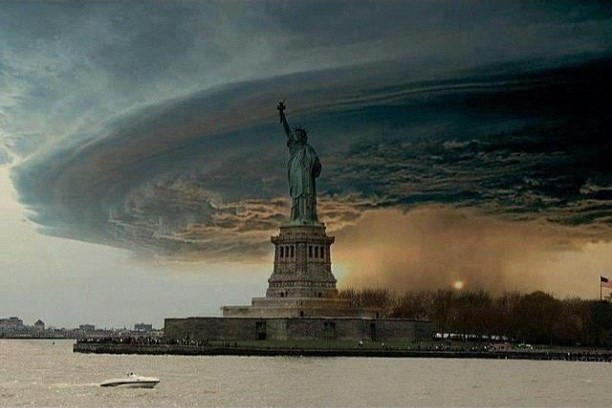
\includegraphics[width=\linewidth]{images/fake_example.jpg}
        \caption{New York gonna be\\screwed \#sandy \#hurricane\\\#newyork \#fucked}
        \label{fig:fake}
    \end{subfigure}
    \hspace*{\fill} % separation between the subfigures
    \begin{subfigure}{0.31\textwidth}
        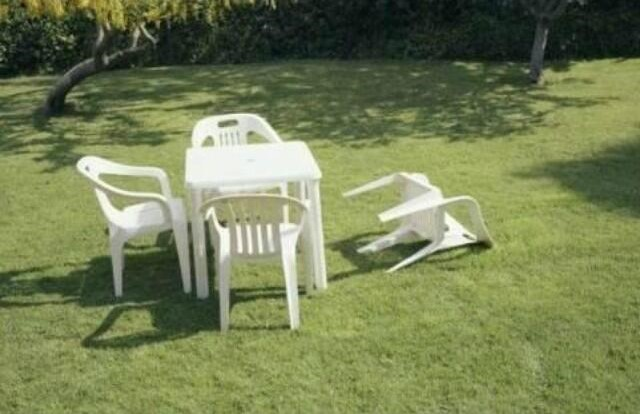
\includegraphics[width=\linewidth]{images/humor_example.jpg}
        \caption{Britain's last hurricane\\was devastating...}
        \label{fig:humor}
    \end{subfigure}
    \caption{当研究で扱う3カテゴリの投稿例: (a)正しいニュース,(b)フェイクニュース,(c)ジョークニュース}
    \label{fig:examples}
\end{figure}

いずれもTwitter上で投稿されたことがある投稿である.
当研究では,こういった投稿を自動で分類することを目指す.
%
\section{達成目標}
%